% conference:  http://www.iros2015.org/
%https://ras.papercept.net/conferences/scripts/start.pl       to submit
% https://ras.papercept.net/conferences/scripts/pdftest.pl  to test pdf

% obstacles: brown
% robots: blue

%(Note: The game industry has picked up on this -- for my NSF propose I talked with ReignGames (who makes Flockwork: Flockwork by ReignGames - YouTube) and included a letter from them.  Similar games are SuperFruitfall and Denki Blocks). 
%Figure 1, Results from 1624 user experiments on block pushing task with the different levels of feedback shown in Fig. 1


\documentclass[letterpaper, 10 pt, conference]{ieeeconf}
\IEEEoverridecommandlockouts
%\documentclass[12pt]{article}
%\usepackage{times}
\usepackage{calc}
\usepackage{url}
\usepackage{hyperref}
\hypersetup{
  colorlinks =true,
  urlcolor = black,
  linkcolor = black
}
\usepackage{graphicx}
\usepackage[cmex10]{amsmath}
\usepackage{bm}
\usepackage{amssymb}
\usepackage{rotating}


%\usepackage{xfrac}
\usepackage{nicefrac}
\usepackage{cite}
\usepackage[caption=false,font=footnotesize]{subfig}
\usepackage[usenames, dvipsnames]{color}
\usepackage{colortbl}
%\usepackage{caption}

%\usepackage{wrapfig}
\usepackage{overpic}
%\usepackage{subfigure}
%\usepackage{textcomp}
\graphicspath{{./pictures/pdf/},{./pictures/ps/},{./pictures/png/},{./pictures/jpg/}}
\usepackage{breqn} %for breaking equations automatically
\usepackage[ruled]{algorithm}
\usepackage{algpseudocode}
%\usepackage{algorithmic}
\usepackage{multirow}
\usepackage{todonotes}

%\newcommand{\todo}[1]{\vspace{5 mm}\par \noindent \framebox{\begin{minipage}[c]{0.98 \columnwidth} \ttfamily\flushleft \textcolor{red}{#1}\end{minipage}}\vspace{5 mm}\par}
% uncomment this to hide all red todos
%\renewcommand{\todo}{}

%% ABBREVIATIONS
\newcommand{\qstart}{q_{\text{start}}}
\newcommand{\qgoal}{q_{\text{goal}}}
\newcommand{\pstart}{p_{\text{start}}}
\newcommand{\pgoal}{p_{\text{goal}}}
\newcommand{\xstart}{x_{\text{start}}}
\newcommand{\xgoal}{x_{\text{goal}}}
\newcommand{\ystart}{y_{\text{start}}}
\newcommand{\ygoal}{y_{\text{goal}}}
\newcommand{\gammastart}{\gamma_{\text{start}}}
\newcommand{\gammagoal}{\gamma_{\text{goal}}}
\providecommand{\proc}[1]{\textsc{#1}}


\newcommand{\ARLfull}{Aero\-space Ro\-bot\-ics La\-bora\-tory }
\newcommand{\ARL}{\textsc{arl}}
\newcommand{\JPL}{\textsc{jpl}}
\newcommand{\PRM}{\textsc{prm}}

\newcommand{\CM}{\textsc{cm}}
\newcommand{\SVM}{\textsc{svm}}
\newcommand{\NN}{\textsc{nn}}
\newcommand{\prm}{\textsc{prm}}
\newcommand{\lemur}{\textsc{lemur}}
\newcommand{\Lemur}{\textsc{Lemur}}
\newcommand{\LP}{\textsc{lp}} 
\newcommand{\SOCP}{\textsc{socp}}
\newcommand{\SDP}{\textsc{sdp}}
\newcommand{\NP}{\textsc{np}}
\newcommand{\SAT}{\textsc{sat}}
\newcommand{\LMI}{\textsc{lmi}}
\newcommand{\hrp}{\textsc{hrp\nobreakdash-2}}
\newcommand{\DOF}{\textsc{dof}}
\newcommand{\UIUC}{\textsc{uiuc}}
%% MACROS


\providecommand{\abs}[1]{\left\lvert#1\right\rvert}
\providecommand{\norm}[1]{\left\lVert#1\right\rVert}
\providecommand{\normn}[2]{\left\lVert#1\right\rVert_#2}
\providecommand{\dualnorm}[1]{\norm{#1}_\ast}
\providecommand{\dualnormn}[2]{\norm{#1}_{#2\ast}}
\providecommand{\set}[1]{\lbrace\,#1\,\rbrace}
\providecommand{\cset}[2]{\lbrace\,{#1}\nobreak\mid\nobreak{#2}\,\rbrace}
\providecommand{\lscal}{<}
\providecommand{\gscal}{>}
\providecommand{\lvect}{\prec}
\providecommand{\gvect}{\succ}
\providecommand{\leqscal}{\leq}
\providecommand{\geqscal}{\geq}
\providecommand{\leqvect}{\preceq}
\providecommand{\geqvect}{\succeq}
\providecommand{\onevect}{\mathbf{1}}
\providecommand{\zerovect}{\mathbf{0}}
\providecommand{\field}[1]{\mathbb{#1}}
\providecommand{\C}{\field{C}}
\providecommand{\R}{\field{R}}
\newcommand{\Cspace}{\mathcal{Q}}
\newcommand{\Uspace}{\mathcal{U}}
\providecommand{\Fspace}{\Cspace_\text{free}}
\providecommand{\Hcal}{$\mathcal{H}$}
\providecommand{\Vcal}{$\mathcal{V}$}
\DeclareMathOperator{\conv}{conv}
\DeclareMathOperator{\cone}{cone}
\DeclareMathOperator{\homog}{homog}
\DeclareMathOperator{\domain}{dom}
\DeclareMathOperator{\range}{range}
\DeclareMathOperator{\sign}{sgn}
\providecommand{\polar}{\triangle}
\providecommand{\ainner}{\underline{a}}
\providecommand{\aouter}{\overline{a}}
\providecommand{\binner}{\underline{b}}
\providecommand{\bouter}{\overline{b}}
\newcommand{\D}{\nobreakdash-\textsc{d}}
%\newcommand{\Fspace}{\mathcal{F}}
\providecommand{\Fspace}{\Cspace_\text{free}}
\providecommand{\free}{\text{\{}\mathsf{free}\text{\}}}
\providecommand{\iff}{\Leftrightarrow}
\providecommand{\subinner}[1]{#1_{\text{inner}}}
\providecommand{\subouter}[1]{#1_{\text{outer}}}
\providecommand{\Ppoly}{\mathcal{X}}
\providecommand{\Pproj}{\mathcal{Y}}
\providecommand{\Pinner}{\subinner{\Pproj}}
\providecommand{\Pouter}{\subouter{\Pproj}}
\DeclareMathOperator{\argmax}{arg\,max}
\providecommand{\Aineq}{B}
\providecommand{\Aeq}{A}
\providecommand{\bineq}{u}
\providecommand{\beq}{t}
\DeclareMathOperator{\area}{area}
\newcommand{\contact}[1]{\Cspace_{#1}}
\newcommand{\feasible}[1]{\Fspace_{#1}}
\newcommand{\dd}{\; \mathrm{d}}
\newcommand{\figwid}{0.22\columnwidth}
\newcommand{\TRUE}{\textbf{true}}
\newcommand{\FALSE}{\textbf{false}}
\DeclareMathOperator{\atan2}{atan2}


\newtheorem{theorem}{Theorem}
\newtheorem{definition}[theorem]{Definition}
\newtheorem{lemma}[theorem]{Lemma}
\begin{document}

%%%%%%%%%%%%%% For debugging purposes, I like to display the TOC
%    \tableofcontents
%    \setcounter{tocdepth}{3}
%\newpage
%\mbox{}
%\newpage
%\mbox{}
%\newpage

%%%%%% END TOC %%%%%%%%%%%%%%%%%%%%%%%%%%%%%%%%%%%%%%%

\title{\LARGE \bf 
Shaping a Swarm Using Wall Friction and a Shared Control Input
}
\author{Shiva Shahrokhi and  Aaron T. Becker%, 
\thanks{{S. Shahrokhi and A. Becker are with the Department of Electrical and Computer Engineering,  University of Houston, Houston, TX 77204-4005 USA {\tt\small  \{sshahrokhi2, atbecker\}@uh.edu}
}
} %\end thanks
} % end author block
\maketitle

\begin{abstract}

Micro- and nano-robots can be manufactured in large numbers. Large numbers of micro robots are required in order to deliver sufficient payloads, but the small size of these robots makes it difficult to perform onboard computation.  Instead, these robots are often controlled by a global, broadcast signal. 
In our previous work we focused on a block-pushing task, where a swarm of robots pushed a larger block through a 2D maze. One surprising result was that humans that only knew the swarm's mean and covariance completed the task faster that humans who knew the position of every robot~\cite{Becker2013b}. 
Inspired by that work, we proved that we can control the mean position of a swarm and that with an obstacle we can control the swarm's position variance ($\sigma_x$ and $\sigma_y$). 
We then wrote automatic controllers which could complete a block pushing task, but these controllers had some limitations~\cite{ShahrokhiIROS2015}. 
One of the limitations was that we could only compress our swarm along the world $x$ and $y$ axes, and could not navigate workspaces with narrow corridors with other orientations. 
One solution to these problems would be a controller that regulates the swarm's position covariance, $\sigma_{xy}$. 
For controlling $\sigma_{xy}$, we prove that the swarm position covariance $\sigma_{xy}$ is controllable given boundaries with non-zero friction. 
We then prove that two orthogonal boundaries with high friction are sufficient to arbitrarily position a swarm of robots. 
We conclude by designing controllers that efficiently regulate $\sigma_{xy}$.
\end{abstract}


%%%%%%%%%%% PAPER OUTLINE
% INTRODUCTION, Related work
%      micro/nano applications
%	open questions in swarm control
% 	difficulties in obtaining experimental data
% Theory:
%% Wall friction shape
%% Control 2 robots
% Simulation:
%% Use wall friction to control covariance 1. Make variances small(feedback), 2. Move Swarm to wall, 3. drag out swarm to achieve covariance(feedback) 4. Move to goal.
%% Algorithm to control position of 2 robots using friction
%%%%%%% Algorithm to control position of n robots using friction
% Experiment
%% Use wall friction to control covariance
%% Algorithm to control position of 2 robots using friction
%%Future Work

%%%%%%%%%%%%%%%
\section{Introduction}\label{sec:Intro}
%This project studies system models and user interfaces for five multi-robot manipulation tasks with large populations of micro- and nanorobots.  We test several system models with different limitations on controllability and observability of the motion controller, and evaluate several different user interfaces.  We conduct user experiments to understand the impact of these limitations and design choices. 


%Micro- and nanorobotics have the potential to revolutionize many applications including targeted material delivery, assembly, and surgery.  The same properties that promise breakthrough solutions---small size and large populations---present unique challenges to generating controlled motion.  
Large populations of micro- and nanorobots are being produced in laboratories around the world, with diverse potential applications in drug delivery and construction \cite{Peyer2013,Shirai2005,Chiang2011}. These activities require robots that behave intelligently.
Limited computation and communication rules out autonomous operation or direct control over individual units; instead we must rely on global control signals broadcast to the entire robot population.  It is not always practical to gather pose information on individual robots for feedback control; the robots might be difficult or impossible to sense individually due to their size and location. However, it is often possible to sense global properties of the group, such as mean position and density.  Finally, many promising applications will require direct human control, but user interfaces to thousands---or millions---of robots is a daunting human-swarm interaction (HSI) challenge. 

Our previous work with over a hundred hardware robots and thousands of simulated robots~\cite{Becker2013b} demonstrated that direct human control of large swarms is possible. Unfortunately, the logistical challenges of repeated experiments with over one hundred robots prevented large-scale tests. To gather better data, we designed a large-scale online game to test how humans interact with large swarms.  These  experiments~\cite{Becker2014e} showed that numerous simple robots responding to global control inputs are directly controllable by a human operator without special training, and that the visual feedback of the swarm state should be very simple in order to increase task performance.


\begin{figure}
\centering
\begin{overpic}[width=\columnwidth *4 /5]{BlockPushing1.png}\end{overpic}
\todo{I like the 'target' symbol, but it is not self-documenting.  We need a legend explaining the min and max variance ellipses, the goal region, the variance, the mean, the object COM, and the target mean position.  I think these are easiest to make in powerpoint.
Please use the same color and line style for the variance min and max as you use in Figure 4.
}
%{blockpushingImageWithMeanAndVarianceOverlay.png}
\caption{\label{fig:bigPictureMeanAndVarianceForSwarm} A swarm of robots, all controlled by the same, uniform force field, can be effectively controlled hybrid controller that knows only the first and second moments of the robot distribution.  Here a swarm of simple robots (blue discs) pushes a green block toward the goal.}
\end{figure}


%\begin{figure}
%\renewcommand{\figwid}{0.32\columnwidth}
%\subfloat[][Vary Number]{\label{fig:VaryNum}
%\begin{overpic}[width =\figwid]{VaryNum.pdf}\end{overpic}}
%%
%\subfloat[][Vary Visual Feedback]{\label{fig:VaryVis}
%\begin{overpic}[width =\figwid]{VaryVisFS.pdf}\end{overpic}
%\begin{overpic}[width =\figwid]{VaryVisMV.pdf}\end{overpic}}\\
%%
%\subfloat[][Vary Control]{\label{fig:VaryControl}
%\begin{overpic}[width =\figwid]{VaryControl.pdf}\end{overpic}}
%%
%\subfloat[][Vary Noise]{\label{fig:VaryNoise}
%\begin{overpic}[width =\figwid]{VaryNoise.pdf}\end{overpic}}
%%
%\subfloat[][Control Position]{\label{fig:ControlPos}
%\begin{overpic}[width =\figwid]{ControlPos.pdf}\end{overpic}}
%%
%\caption{\label{fig:5experiments}
%Screenshots from our five online experiments controlling multi-robot systems with limited, global control.
%\textbf{(a)} Varying the number of robots from 1-500
%\textbf{(b)} Comparing 4 levels of visual feedback 
%\textbf{(c)} Comparing 3 control architectures
%\textbf{(d)} Varying noise from 0 to 200\% of control authority
%\textbf{(e)} Controlling the position of 1 to 10 robots.
%\href{http://youtu.be/HgNENj3hvEg}{See video overview at http://youtu.be/HgNENj3hvEg.}
%\vspace{-2em}
%}
%\end{figure}






% Our paper is organized as follows.  After a discussion of related work in Section \ref{sec:RelatedWork}, we describe our experimental methods for an online human-user experiment in Section \ref{sec:expMethods}.  We report the results of our experiments in Section \ref{sec:expResults}, discuss the lessons learned in Section \ref{sec:discussion}, and end with concluding remarks in Section \ref{sec:conclusion}.



%%%%%%%%%%%%%%%
%%%%%%%%%%%%%%%
%%%%%%%%%%%%%%%%%%%%%%%%%%%%%%%%%%%%%%%%%%%%%%%%%%%%%%%%%%%
\section{Theory}
\label{sec:theory}
%%%%%%%%%%%%%%%%%%%%%%%%%%%%%%%%%%%%%%%%%%%%%%%%%%%%%%%%%%%
\subsection{Controlling covariance using friction}
Global inputs move a swarm uniformly.  
Controlling covariance requires breaking this uniform symmetry.  A swarm inside an axis-aligned rectangular workspace can reduce variance normal to a wall by simply pushing the swarm into the boundary. Directly controlling covariance by pushing the swarm into a boundary requires changing the boundary.  An obstacle in the lower-right corner is enough to generate positive covariance.  Generating both positive and negative covariance requires additional obstacles.  Requiring special obstacle configuration also makes covariance control dependent on the local environment. 
  Instead of pushing our robots directly into a wall, this paper examines an oblique approach, by using boundaries that generate friction with the robots.  These frictional forces are  sufficient to break the symmetry caused by uniform inputs.  Robots touching a wall have a negative friction force that opposes movement along the boundary, as shown in Eq.\ \eqref{eq:frictionmodel}.  This  causes robots along the boundary to slow down compared to robots in free-space. This enables covariance control using  boundaries with arbitrary orientations. 
  
 Let the control input be a vector force $\vec{F}$ with magnitude $F$ and orientation $\theta$.  The force of friction $F_f$ is
\begin{align}
N &= F \cos(\theta) \nonumber\\
F_f &= \begin{cases}  \mu_f N, &  \mu_f N < F \sin(\theta)  \label{eq:frictionmodel} \\ 
F \sin(\theta), & \text{else} \end{cases}  \\%\sign(F \sin(\theta) ) \cdot  \max(0, | F sin\theta |- |F_f|)
F_{\text{\emph{forward}}} &=  F \sin(\theta) - F_f  \nonumber
\end{align}
 Fig.~\ref{fig:friction} shows the resultant forces on two robots when one is touching a wall. As illustrated, bot experiences different net forces although each receive the same inputs.
  For ease of analysis, the following algorithms assume $\mu_f$ is infinite and robots touching the wall are prevented from sliding along the wall.
This means that if one robot is touching the wall and another robot is free, if the control input is parallel or into the wall, the touching robot will not move. 
The next section shows how a system with friction model \eqref{eq:frictionmodel} and two walls are sufficient to arbitrarily position two robots. 
\begin{figure}[h]
\begin{center}
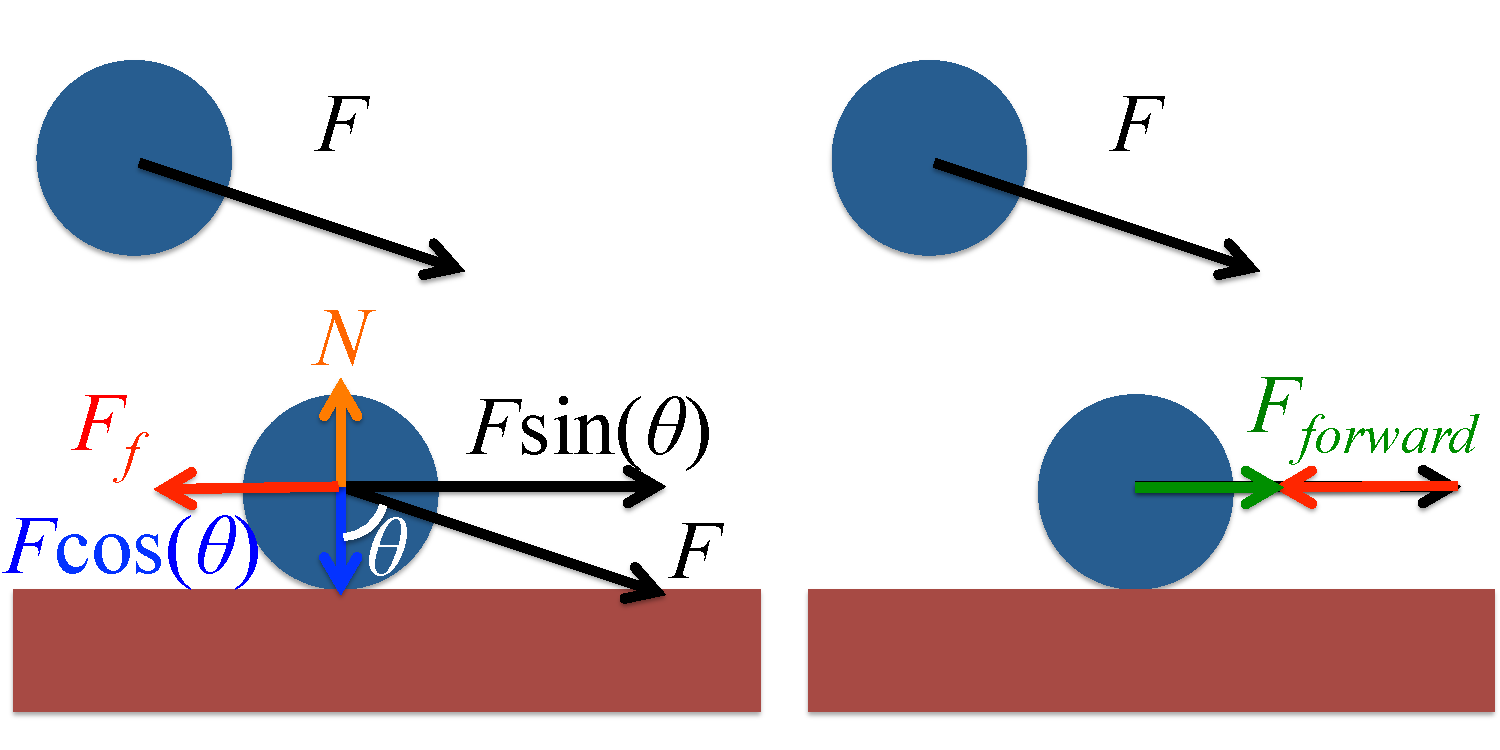
\includegraphics[width=\columnwidth]{friction.pdf} 
\caption{Wall friction reduces the force for going forward $F_{\text{\emph{forward}}}$ on a robot near a wall, but not for a free robot.}
\label{fig:friction}
\end{center}
\end{figure} 




\section{Position control of $2$ robots using wall friction}\label{sec:PostionControl2Robots}
This section describes an algorithm for positioning two robots and introduces concepts that will be used for multi-robot positioning.
%Although the generalization of the proposed positioning algorithm in here is rather straightforward for multi robot systems, for the sake of simplicity we describe the algorithm designed for two robots. 
As we can see from Alg.~\ref{alg:PosControl2Robots}, assume two robots are initialized at $s_1$ and $s_2$ with corresponding goal destinations $e_1$ and $e_2$. 
Denote the current positions of the robots  $r_1$ and $r_2$. 
Let the subscripts $x$ and $y$ denote the $x$ and $y$ coordinates, i.e., $s_{1x}$ and $s_{1y}$ denote the $x$ and $y$ locations of $s_1$. 
The algorithm assigns a global control input at every instance.
 As a result, our goal is to adjust 
 $\Delta r_x = r_{2x}-r_{1x}$ from $\Delta s_x = s_{2x}-s_{1x}$ to $\Delta e_x = e_{2x}-e_{1x}$ and similarly adjust 
 $\Delta r_y = r_{2y}-r_{1y}$ from $\Delta s_y = s_{2y}-s_{1y}$ to $\Delta e_y = e_{2y}-e_{1y}$ with one global input at every instance. 
 The key to the algorithm is the position-dependent friction model \eqref{eq:frictionmodel}.
 %employing the assumption we have made earlier about the walls' friction. 

Our algorithm uses a divide and conquer method to solve the positioning problem. 
It finds the final position of the robots in two steps: (i) First, $|\Delta r_x - \Delta e_x |$ is reduced to zero while  $\Delta r_y$ is kept constant in Alg.~\ref{alg:XControl}. 
(ii) Having fixed $\Delta r_x$ to $\Delta e_x$ as desired, the  algorithm next keeps $\Delta r_x$ constant and adjusts $\Delta r_y$ to $\Delta e_y$, as desired in Alg..~\ref{alg:YControl}. 
Though steps (i) and (ii) are similar from an algorithmic point of view, the following subsections describe the process in detail. 

\subsection{Step (i): Fixing $\Delta r_x$}
\label{theory:step1}
\begin{itemize}
\item Define $e'_1=(e_{1x},s_{1y})$ and $e'_2=(e_{2x},s_{2y})$. Our goal for defining $e'_1$ and $e'_2$ is to understand the direction to which robots should move in order to adjust $\Delta r_x$. Let $e'_{\rm{top}} = \arg \max_i e'_{iy}$ and $e'_{\rm{bottom}} = \arg \min_i e'_{iy}$. Now if $e'_{\rm{top},x}-e'_{\rm{bottom},x}>0$, then the global input to both robots would be toward left direction and if $e'_{\rm{top},x}-e'_{\rm{bottom},x}<0$, then the global input to both robots would be toward right direction. The two robots continue their horizontal path until one of them reaches the $\epsilon$-neighborhood of one of the left or right walls.
\item At this step, let $y_{\min} = \min_i r_{iy}$, i.e., $y_{\min}$ is the minimum height of the two robots. We move both robots downward by the amount of $y_{\min}$ such that one of the robots would touch the bottom wall and hence friction force will not let that robot to move left or right.
\item The fact that the friction force of the bottom wall would not let the lower robot to move right or left will let the other robot to move to right and left freely to adjust $\Delta r_x $ according to $\Delta e_x$.
\item Finally, even if with the free move of the upper robot $\Delta r_x$ is not set to the $\Delta e_x$, we can run the Step (i) (as described in the previous paragraphs) again to adjust the $\Delta r_x$. It is easy to show that it is guaranteed that we can adjust $\Delta r_x$ to $\Delta e_x$ in only two iterations.
\end{itemize}

\subsection{Step (ii): Fixing $\Delta r_y$}
Now that we have adjusted the difference in robots' positions along one axis, we focus to do the same on the other axis as well. Therefore, similar to Section \ref{theory:step1}, we employ the following steps:
\begin{itemize}
\item Let $s'_1$ and $s'_2$ be the points we derived at the end of the steps in Section \ref{theory:step1}. 
\item Define $e''_1=(s'_{1x},e_{1y})$ and $e''_2=(s'_{2x},e_{2y})$. We define $e''_1$ and $e''_2$ to understand the direction to which robots should move in order to adjust $\Delta r_y$. Let $e''_{\rm{right}} = \arg \max_i e''_{ix}$ and $e''_{\rm{left}} = \arg \min_i e'_{ix}$. Now if $e''_{\rm{right},y}-e''_{\rm{left},y}>0$, then the global input to both robots would be toward down direction and if $e''_{\rm{right},y}-e''_{\rm{left},y}<0$, then the global input to both robots would be toward up direction. The two robots continue their vertical path until one of them reaches the $\epsilon$-neighborhood of one of the top or bottom walls.
\item At this step, let $x_{\min} = \min_i r_{ix}$, i.e., $x_{\min}$ is the minimum distance of the two robots from the origin along the $x$-axis. We move both robots to the left by the amount of $x_{\min}$ such that one of the robots would touch the left wall and hence friction force will not let that robot to move up or down.
\item The fact that the friction force of the left wall would not let one of the robots to move up or down will let the other robot to move to up or down freely to adjust $\Delta r_y $ according to $\Delta e_y$.
\item Finally, even if with the free move of the robot which is not touching the wall  $\Delta r_y$ is not set to the $\Delta e_y$, we can run the Step (i) (as described in the previous paragraphs) again to adjust the $\Delta r_y$. It is easy to show that it is guaranteed that we can adjust $\Delta r_y$ to $\Delta e_y$ in only two iterations.
\end{itemize}
Once $\Delta r_x$ and $\Delta r_y$ are set to $\Delta e_x$ and $\Delta e_y$, we can use global input to easily move both robots from $r_1$ and $r_2$ toward $e_1$ and $e_2$. 


\begin{algorithm}
\caption{WallFrictionArrange2Robots($s_1,s_2,e_1,e_2,L$)}\label{alg:PosControl2Robots}
\begin{algorithmic}[1]
\Require 
Knowledge of starting $(s_1,s_2)$ and ending $(e_1,e_2)$ positions of  two robots. 
$(0,0)$ is bottom corner, $s_1$ is rightmost robot, 
 $L$ is length of the walls. 
 Current position of the robots are $(r_1,r_2)$.

\State ($r_1,r_2$) = GenerateDesired$x$-spacing($s_1,s_2,e_1,e_2,L$)
\State GenerateDesired$y$-spacing($r_1,r_2,e_1,e_2,L$)

\end{algorithmic}
\end{algorithm}


\begin{algorithm}
\caption{GenerateDesired$x$-spacing($s_1,s_2,e_1,e_2,L$)}\label{alg:XControl}
\begin{algorithmic}[1]
\Require Knowledge of starting $(s_1,s_2)$ and ending $(e_1,e_2)$ positions of  two robots. 
$(0,0)$ is bottom corner, $s_1$ is topmost robot, 
 $L$ is length of the walls. Current robot positions are $(r_1,r_2)$.
\Ensure   $ r_{1y} - r_{2y}  \equiv s_{1y} - s_{2y} $   %$\Delta y(t) \equiv \Delta y(0)$ 
\State $\epsilon \gets $ small number
\State $ \Delta s_x  \gets s_{1x} - s_{2x} $
\State $ \Delta e_x \gets e_{1x} - e_{2x} $
\State $ r_1 \gets s_1$, $ r_2 \gets s_2$
\If {$\Delta e_x < 0 $ }
\State $ m \gets ( L-\epsilon-\max( r_{1x},r_{2x}) ,0)   $ \Comment{Move to right wall}
\Else 
\State  $ m \gets ( \epsilon-\min( r_{1x},r_{2x}),0 )    $ \Comment{Move to left wall}
\EndIf
\State $m  \gets  m + (0, -\min( r_{1y},r_{2y} ))$ \Comment{Move to bottom}
\State $ r_1 \gets r_1+m$, $ r_2 \gets r_2+m$ \Comment{Apply move}
\If {$\Delta e_x - (r_{1x} - r_{2x} ) > 0 $}
\State $ m \gets (\min(|\Delta e_x - \Delta s_x |, L- r_{1x}), 0)$  \Comment{Move right}
\Else
\State $ m \gets (-\min(|\Delta e_x - \Delta s_x |, r_{1x}), 0)$\Comment{Move left}
\EndIf 
\State $m  \gets  m + (0, \epsilon)$ \Comment{Move up}
\State $ r_1 \gets r_1+m$, $ r_2 \gets r_2+m$ \Comment{Apply move}
\State $\Delta r_x = r_{1x} - r_{2x}$
\If {$\Delta r_x \equiv \Delta e_x$} 
%\State   $ m \gets (e_{1x}-r_{1x}, e_{1y}-r_{1y})$
%\State $ r_1 \gets r_1+m$, $ r_2 \gets r_2+m$ \Comment{Apply move}
\State  \Return $(r_1,r_2)$
\Else   
\State \Return GenerateDesired$x$-spacing($r_1,r_2,e_1,e_2,L$)
\EndIf
\end{algorithmic}
\end{algorithm}

\begin{algorithm}
\caption{GenerateDesired$y$-spacing($s_1,s_2,e_1,e_2,L$)}\label{alg:YControl}
\begin{algorithmic}[1]
\Require Knowledge of starting $(s_1,s_2)$ and ending $(e_1,e_2)$ positions of  two robots. 
$(0,0)$ is bottom corner, $s_1$ is rightmost robot, 
 $L$ is length of the walls. Current position of the robots are $(r_1,r_2)$.
\Ensure   $ r_{1x} - r_{2x}  \equiv s_{1x} - s_{2x} $   %$\Delta y(t) \equiv \Delta y(0)$ 
\State $ \Delta s_y  \gets s_{1y} - s_{2y} $
\State $ \Delta e_y \gets e_{1y} - e_{2y} $
\State $ r_1 \gets s_1$, $ r_2 \gets s_2$
\If {$\Delta e_y < 0 $ }
\State $ m \gets ( L-\max( r_{1y},r_{2y}) ,0)   $ \Comment{Move to top wall}
\Else 
\State  $ m \gets ( -\min( r_{1y},r_{2y}),0 )    $ \Comment{Move to bottom wall}
\EndIf
\State $m  \gets  m + (0, -\min( r_{1x},r_{2x} ))$ \Comment{Move to left}
\State $ r_1 \gets r_1+m$, $ r_2 \gets r_2+m$ \Comment{Apply move}
\If {$\Delta e_y - (r_{1y} - r_{2y} ) > 0 $}
\State $ m \gets (\min(|\Delta e_y - \Delta s_y |, L- r_{1y}), 0)$  \Comment{Move top}
\Else
\State $ m \gets (-\min(|\Delta e_y - \Delta s_y |, r_{1y}), 0)$\Comment{Move bottom}
\EndIf 
\State $m  \gets  m + (0, \epsilon)$ \Comment{Move right}
\State $ r_1 \gets r_1+m$, $ r_2 \gets r_2+m$ \Comment{Apply move}
\State $\Delta r_y = r_{1y} - r_{2y}$
\If {$\Delta r_y \equiv \Delta e_y$} 
\State   $ m \gets (e_{1x}-r_{1x}, e_{1y}-r_{1y})$
\State $ r_1 \gets r_1+m$, $ r_2 \gets r_2+m$ \Comment{Apply move}
\State  \Return $(r_1,r_2)$
\Else   
\State \Return GenerateDesired$y$-spacing($r_1,r_2,e_1,e_2,L$)
\EndIf
\end{algorithmic}
\end{algorithm}






\section{Position Control of $n$ robots using wall friction}\label{sec:PostionControlnRobots}
Algorithm \ref{alg:PosControl2Robots}  can be extended to control the position of $n$ robots using wall friction under several constraints. The solution described here is an iterative procedure with $n$ loops. The $k$th loop moves the $k$th robot from staging zone to the desired position in a build zone. At the end the $k$th loop, robots 1 through $k$ are in their desired final configuration in the build zone, and robots $k+1$ to $n$ are in the staging zone.

Assume an open workspace with four axis-aligned walls with infinite friction.

\begin{figure}
\begin{center}
	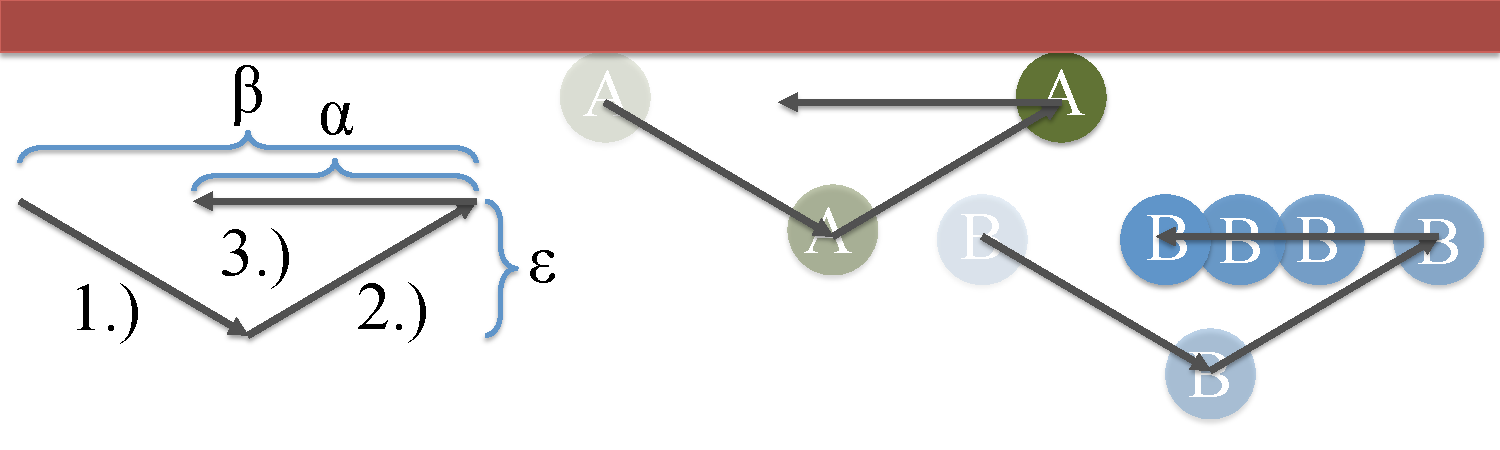
\includegraphics[width=1.0\columnwidth]{driftmove.pdf}
\end{center}
\caption{\label{fig:driftmove}
A  $\operatorname{DriftMove}(\alpha, \beta, \epsilon)$ consists of repeating a triangular movement sequence $\{ (\beta/2,-\epsilon),(\beta/2,\epsilon),(-\alpha,0)\}$. The robot $A$ touching a top wall will move right $\beta$ units, while robots not touching the top move right $\beta-\alpha$.
}
\end{figure}



The axis-aligned build zone of dimension $(w_b, h_b)$ containing the final configuration of $n$ robots must be disjoint from the axis-aligned staging zone of dimension $(w_s, h_s)$  containing the starting configuration of $n$ robots. Without loss of generality, assume the build zone  is above the staging zone . 
Furthermore, there must be at least $\epsilon$ space above the build zone, $\epsilon$ below the staging zone , and $\epsilon + 2r$ to the left of the build and staging zone, where $r$ is the radius of a robot.  The minimum workspace is then $(\epsilon + 2r + \max(w_f,w_s), 2\epsilon + h_s,h_f)$.

The $n$ robot position control algorithm relies on a $\operatorname{DriftMove}(\alpha, \beta, \epsilon)$ control input, shown in Fig.\  \ref{fig:driftmove}.
A drift move consists of repeating a triangular movement sequence $\{ (\beta/2,-\epsilon),(\beta/2,\epsilon),(-\alpha,0)\}$. The robot $A$ touching a top wall moves right $\beta$ units, while robots not touching the top move right $\beta-\alpha$.

Let $(0,0)$ be the lower left corner of the workspace, $p_k$ the $x,y$ position of the $k$th robot, and $f_k$ the final $x,y$ position of the $k$th robot. Label the robots in the staging zone from left-to-right and top-to-bottom, and the $f_k$ configurations right-to-left and top-to-bottom as shown in Fig.~\ref{fig:construction2d}.

\begin{algorithm}
\caption{PositionControl$n$RobotsUsingWallFriction($k$)}\label{alg:PosControlNRobots}
\begin{algorithmic}[1]
\State move( $-\epsilon, r-p_{k,y}$) % move  away from right wall and down till robot k touches bottom


\While{ $p_{k,x} > r$} 
\State $\operatorname{DriftMove}(0, \min(p_{k,x} - r,\epsilon), \epsilon)$ left   %drift move left until kth robot touches left wall
\EndWhile

\State $m \gets \operatorname{ceil}\frac{f_{ky}-r}{\epsilon}$
\State $\beta \gets \frac{f_{ky}-r}{m}$
\State $\alpha \gets \beta - \frac{\epsilon}{m}$
\For{ $m$ iterations}
\State $\operatorname{DriftMove}(\alpha, \beta, \epsilon)$ up   %move kth robot to f_{ky} and leave the rest in position.
\EndFor

\State move($r+\epsilon-f_{kx}, 0$)  % move the group to the left until k is in the correct relative x position
\State move($f_{kx}-r, 0$)  

\end{algorithmic}
\end{algorithm}
Algorithm \ref{alg:PosControlNRobots} procedes as follows:  
First, the robots are moved  away from right wall and down so robot $k$ touches bottom.
Second, a set of $\operatorname{DriftMove()}$s are executed that  move the $k$ robot to the left wall with no net movement on the other robots.
Third, a set of $\operatorname{DriftMove()}$s are executed that  move the $k$ robot to it's target height and return the other robots to their initial heights. 
Fourth, all robots except the $k$ robot are pushed left until the $k$ robot is in the correct relative $x$ position compared to robots 1 to $k-1$.
Finally, all robots are moved right until robot $k$ is in the desired target position.
\begin{figure}
\begin{center}
	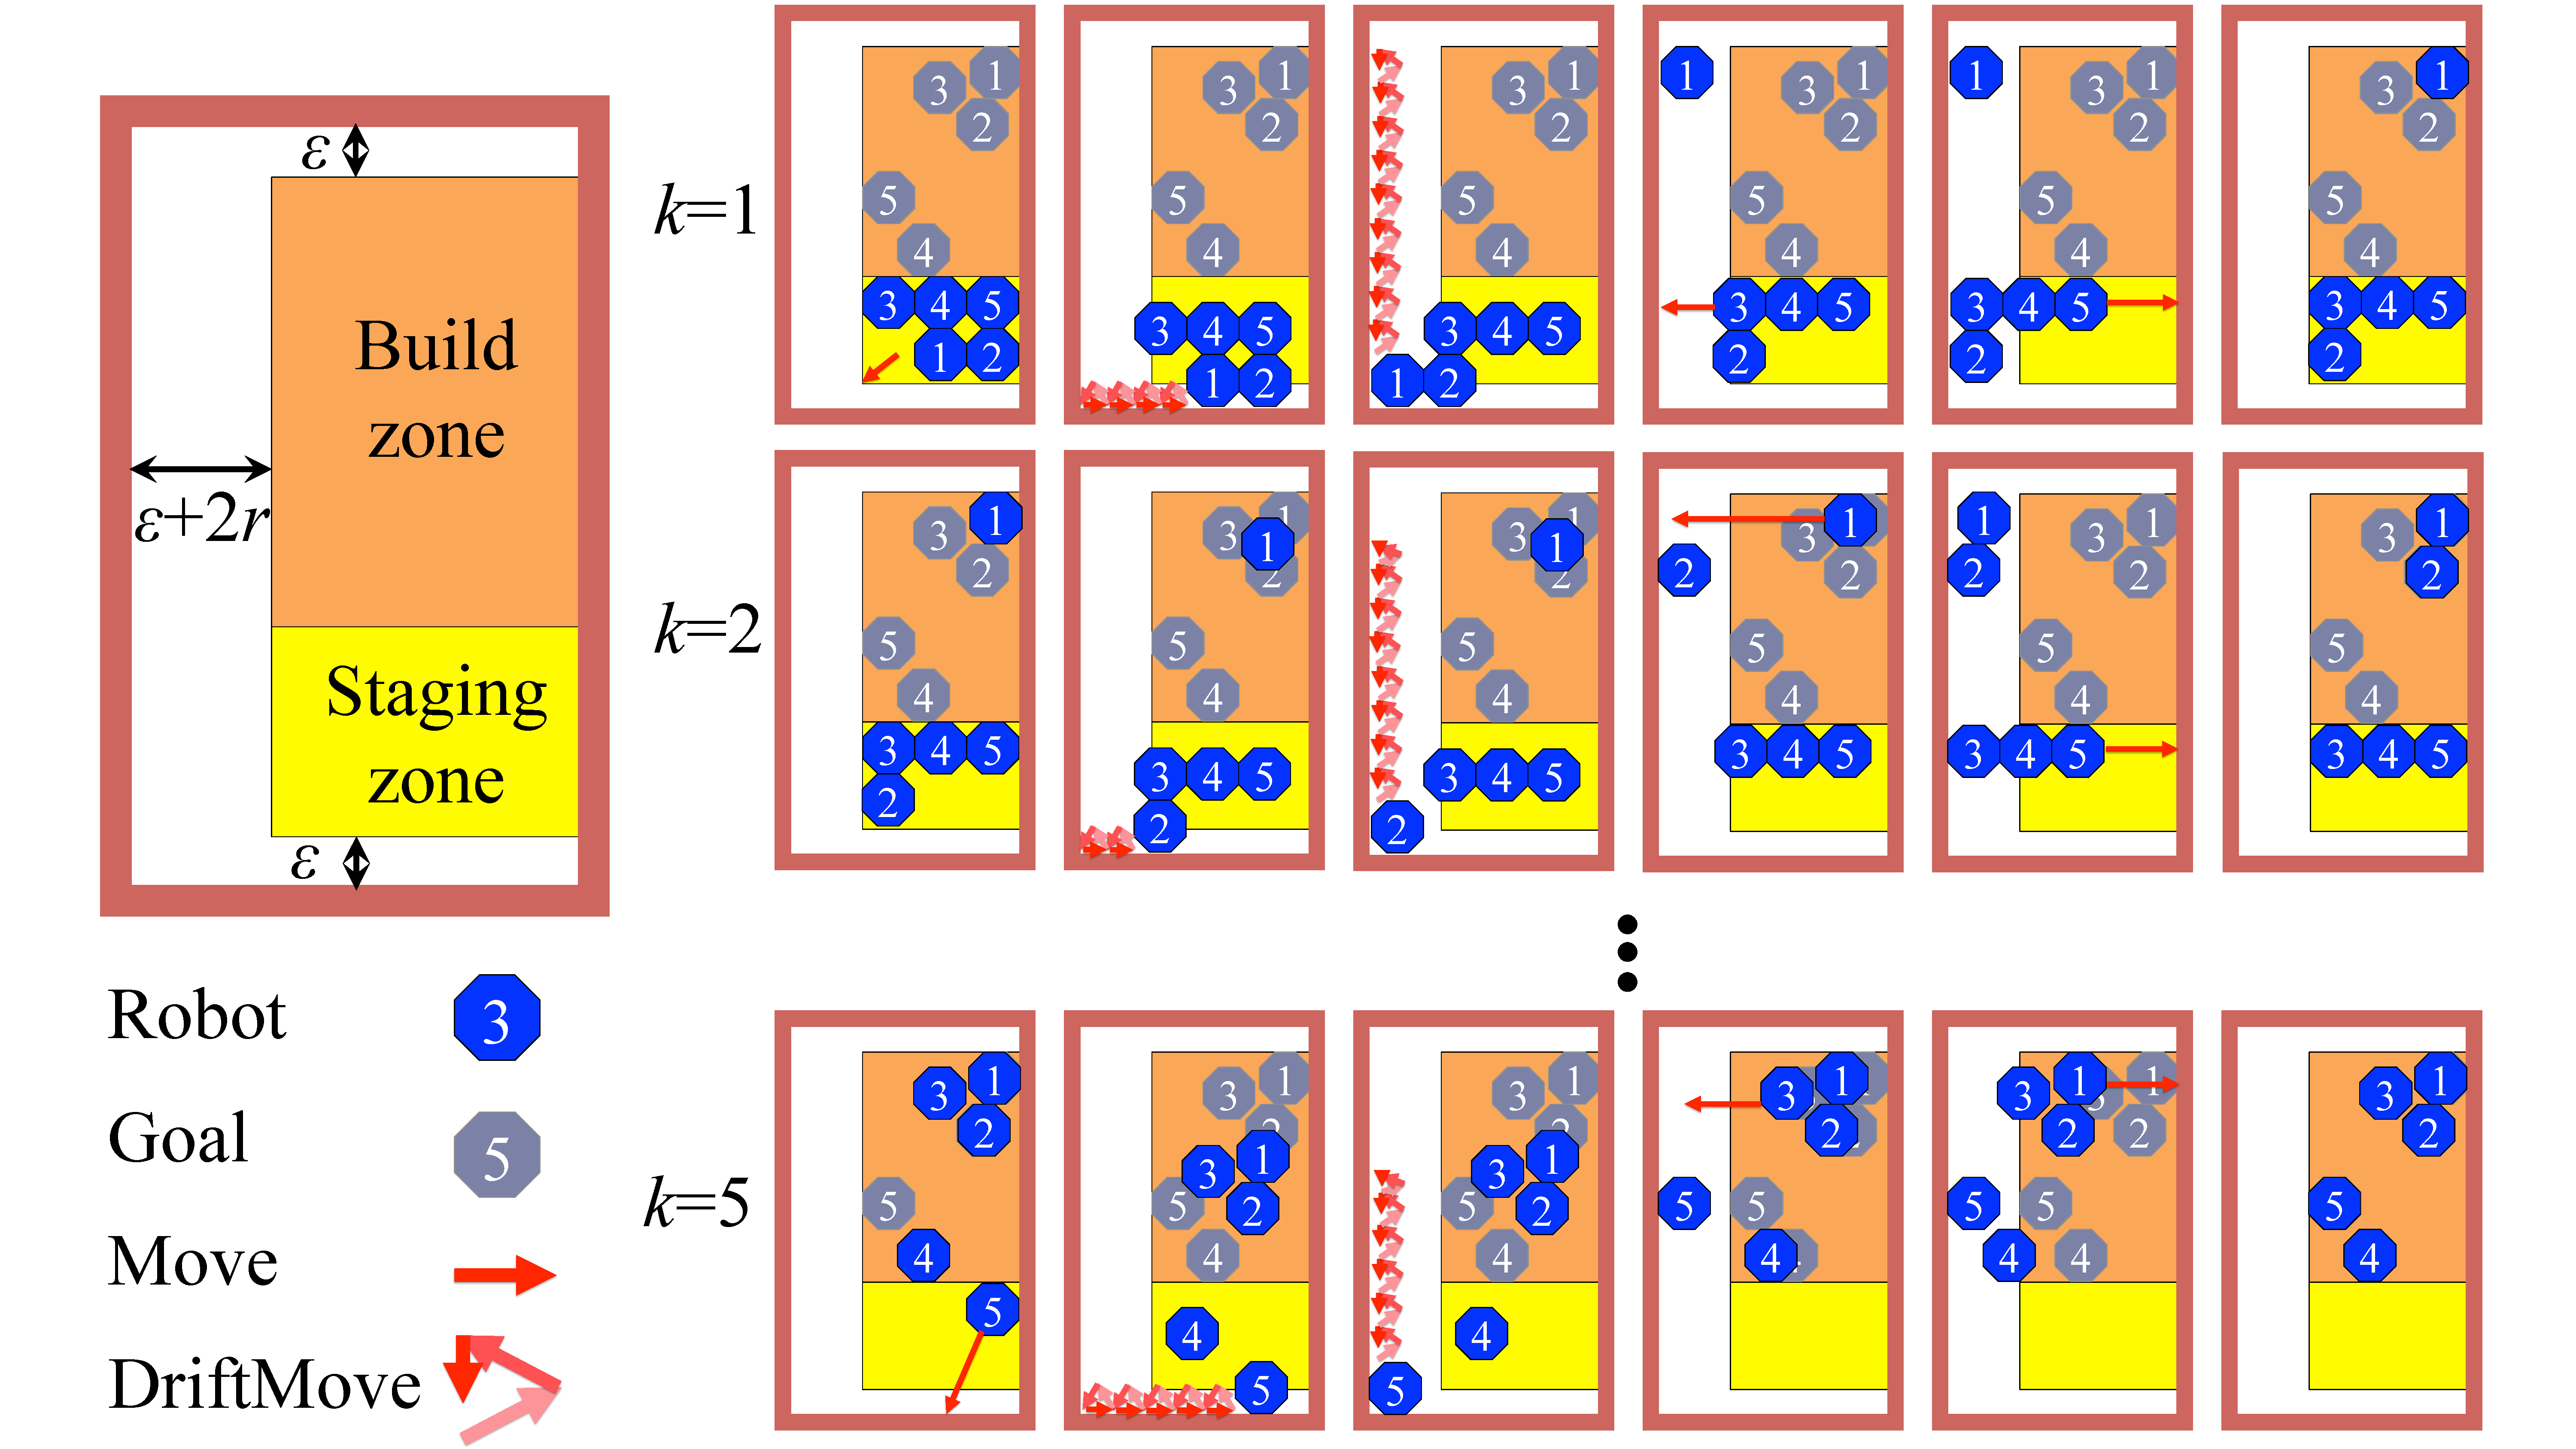
\includegraphics[width=1.0\columnwidth]{PositionNrobots.pdf}
\end{center}
\caption{\label{fig:construction2d}
Illustration of Alg.\ \ref{alg:PosControlNRobots}, $n$ robot position control  using wall friction.
}
\end{figure}














%%%%%%%%%%%%%%%
%%%%%%%%%%%%%%%

\section{Simulation}\label{sec:simulation}

Two simulations were implemented using wall-friction for position control.  The first controls the position of two robots, the second controls the position of $n$ robots.  All code is available online at [link withheld for review].

Two additional simulations were performed using wall-friction to control variance and covariance.  The first is an open-loop algorithm that demonstrates the effect of varying friction levels.  The second uses a closed-loop controller to achieve desired variance and covariance values.



\subsection{Position Control of Two Robots}

Algorithms \ref{alg:PosControl2Robots}, \ref{alg:XControl}, \ref{alg:YControl}, were implemented in Mathematica using point robots (radius = $0$).  Fig.~\ref{fig:shapeControlMathematica1}  shows  this algorithm for two configurations. 
Robot initial positions are shown by a crosshair, and final positions by a circled crosshair.  Dashed lines show the shortest route if robots could be controlled independently.  The path given by  Alg.\ \ref{alg:PosControl2Robots} is shown with solid arrows.
Each row has five snapshots taken every quarter second. For the sake of brevity axis-aligned moves were replaced with oblique moves that combine two moves simultaneously. 
 $\Delta r_x$ is adjusted to $\Delta e_x$ in the second snapshot at $t = 0.25$. 
 The following frames  adjust $\Delta r_y$ to $\Delta e_y$. 
 $\Delta r_y$ is corrected by $t = 0.75$. 
 Finally, the algorithm moves the robots to their corresponding destinations.

In the worse case, adjusting both $\Delta r_x$ and $\Delta r_y$ requires two iterations.   Two iterations of Alg. \ref{alg:XControl} are only required if $|\Delta e_x - \Delta s_x|>L$. 
Similarly,  two iterations of Alg. \ref{alg:YControl} are only required if $|\Delta e_y - \Delta s_y|>L$.


%\textcolor{red}{Shiva:  what is the complexity of this algorithm?  How many steps in the worst case?  When does worst case happen?}
%\begin{figure*}
%\centering
%\renewcommand{\figwid}{0.4\columnwidth}
%{\begin{overpic}[width =\figwid]{one_1.jpg}\put(45,75){$t$ = 0 s}
%\end{overpic}
%\begin{overpic}[width =\figwid]{one_2.jpg}\put(45,75){$t$ = 0.25 s}
%\end{overpic}
%\begin{overpic}[width =\figwid]{one_3.jpg}\put(45,75){$t$  = 0.5 s}
%\end{overpic}
%\begin{overpic}[width =\figwid]{one_4.jpg}\put(45,75){$t$  = 0.75 s}
%\end{overpic}
%\begin{overpic}[width =\figwid]{one_5.jpg}\put(45,75){$t$  = 1 s}
%\end{overpic}}
%\vspace{-1em}
%\caption{\label{fig:shapeControlMathematica2}{Two robot positioning: switching positions using walls with infinite friction.}
%%\vspace{-2em}
%}
%\end{figure*}


\subsection{Position Control of $n$ Robots}
Algorithm \ref{alg:PosControlNRobots}  was simulated in {\sc Matlab} using square block robots with unity width.
Simulation results are shown in Fig.~\ref{fig:4diagramsplots.pdf} for arrangements with an increasing number of robots,  $n$= [8, 46, 130, 390, 862]. 
The distance moved grows quadratically with the number of robots $n$. A best-fit line $210 n^2 + 1200n-10,000$ is overlaid by the data..

In Fig.~\ref{fig:4diagramsplots.pdf}, the amount of clearance $\epsilon=1$.
Control performance is sensitive to the desired clearance.  As $\epsilon$ increases, the total distance decreases asymptotically, as shown in Fig.~\ref{fig:graphrobo.pdf}, because the robots have more room to maneuver and less $\operatorname{DriftMove}$s are required.
%We observed that the value of �?�, greatly affects the total number of moves of commanded moves on the robots. The smaller the value of �?� the greater is the number of moves required to move a said distance. The second graph plot(fig roboplot) is that of �?� vs �total commanded moves� which is the number of moves the global controller commands onto all the robots. Here we take the pattern 
%�ROBO� and calculate the �total commanded moves� for �?�=[ 0.25,0.375,0.5,0.625,0.75,0.875,1]. We can notice an exponential fall in the total command moves. It can be inferred that there is a tradeoff between area of bounded region and the number of moves. For smaller �?�, smaller is the required area to implement algorithm but the longer is the time taken to complete the algorithm. Fig robo
%Unit of �?� is the ratio of minimum clearance value to the body length of a robot.



%The total commanded distance is plotted, which is approximately -0.15v^3 + 385x^2-35000x+300000
%We compare the total distance moved and commanded  with the  \emph{LAP distance}---the shortest distance according to the Linear Assignment Problem using Manhattan distance.   Because all robots are interchangeable, the LAP distance reduces to \[ \text{LAP} =   \sum_{k=1}^n  \left| f_{k,x}-p_{k,x} \right| +  \left|  f_{k,y}-p_{k,y}  \right| . \]


\begin{figure}
\begin{center}
	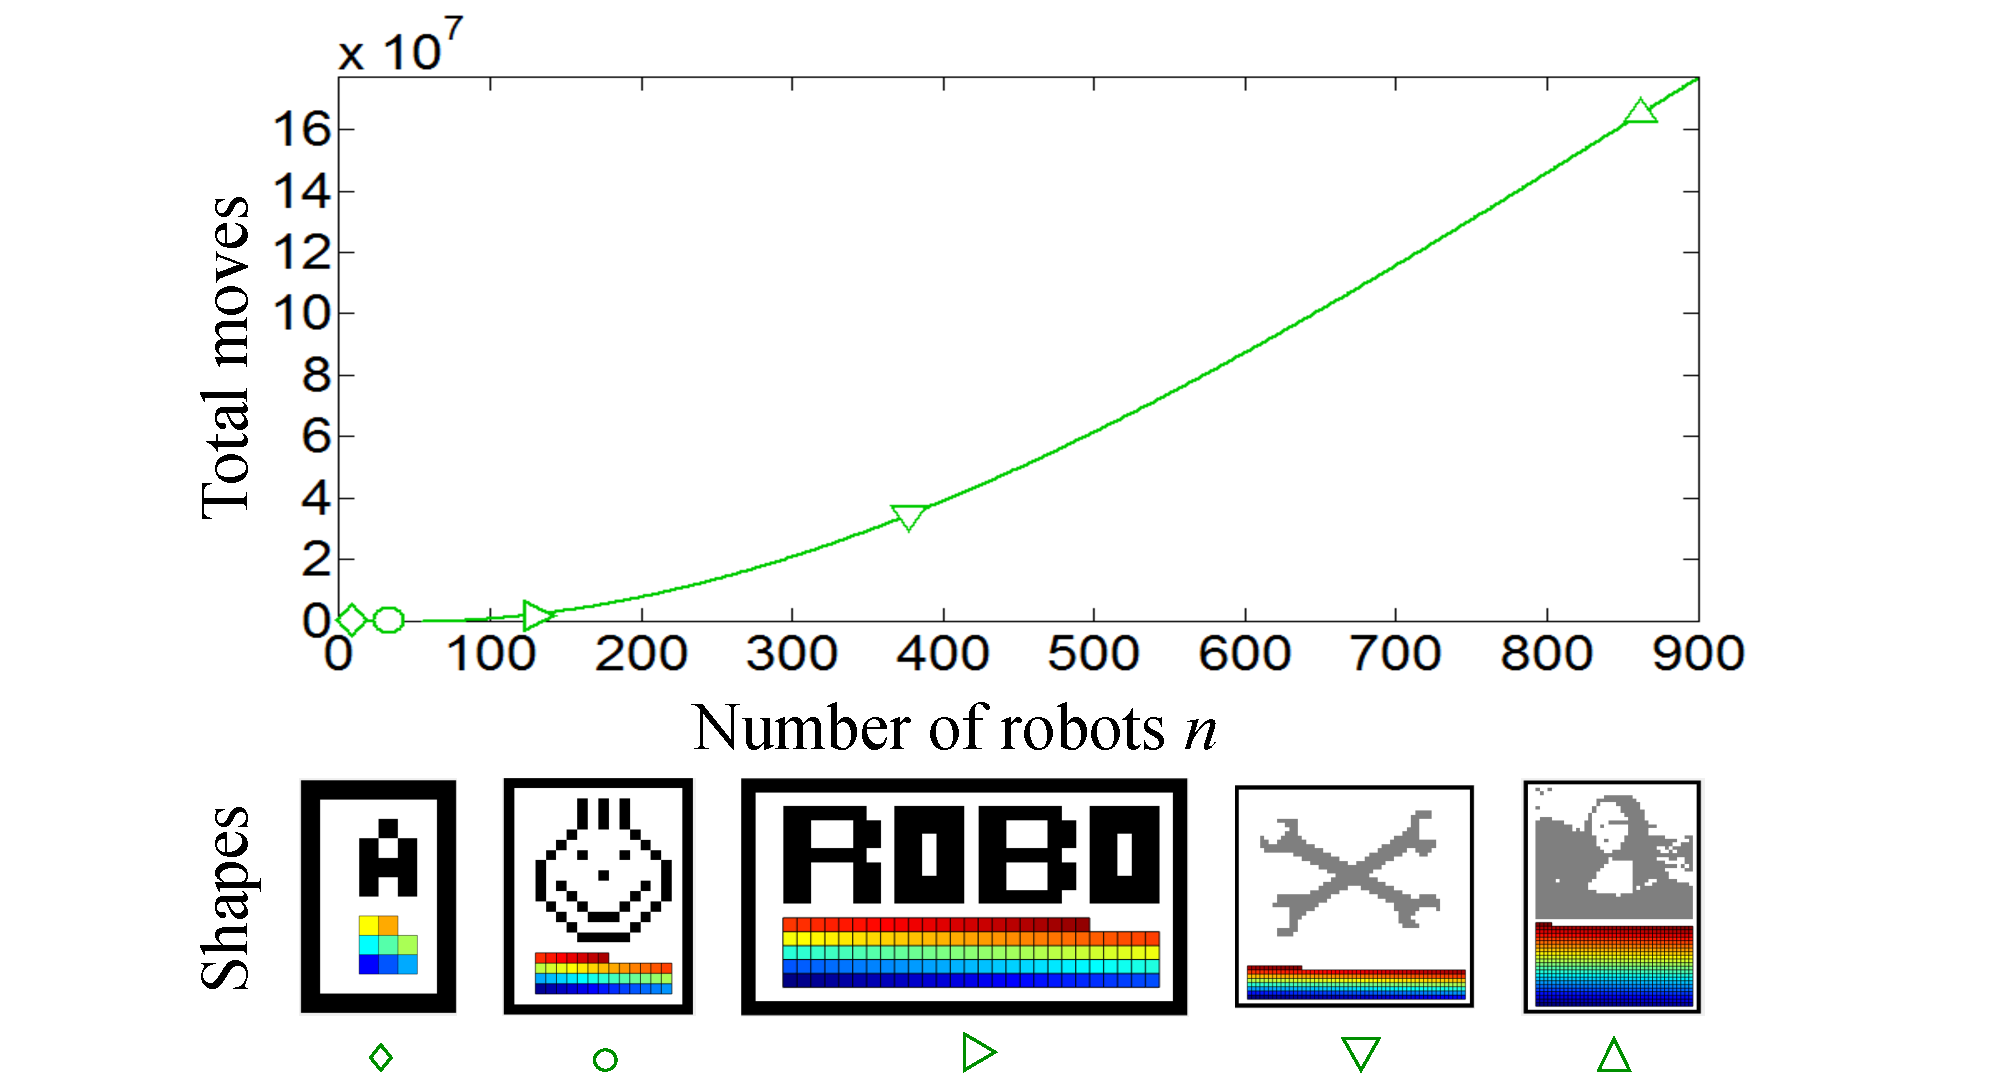
\includegraphics[width=\columnwidth]{5diagramsplots2.pdf}
\end{center}
\caption{\label{fig:4diagramsplots.pdf}
The required number of moves under Algorithm \ref{alg:PosControlNRobots}  using wall-friction to rearrange $n$ square-shaped 
robots.  %The plot compares  \emph{Total distance}---the sum of the moves made by every robot, with \emph{LAP distance}---the shortest distance according to the Linear Assignment Problem using Manhattan distance.  
See hardware implementation and simulation at [link withheld for review].
}
\end{figure}

\begin{figure}
\begin{center}
	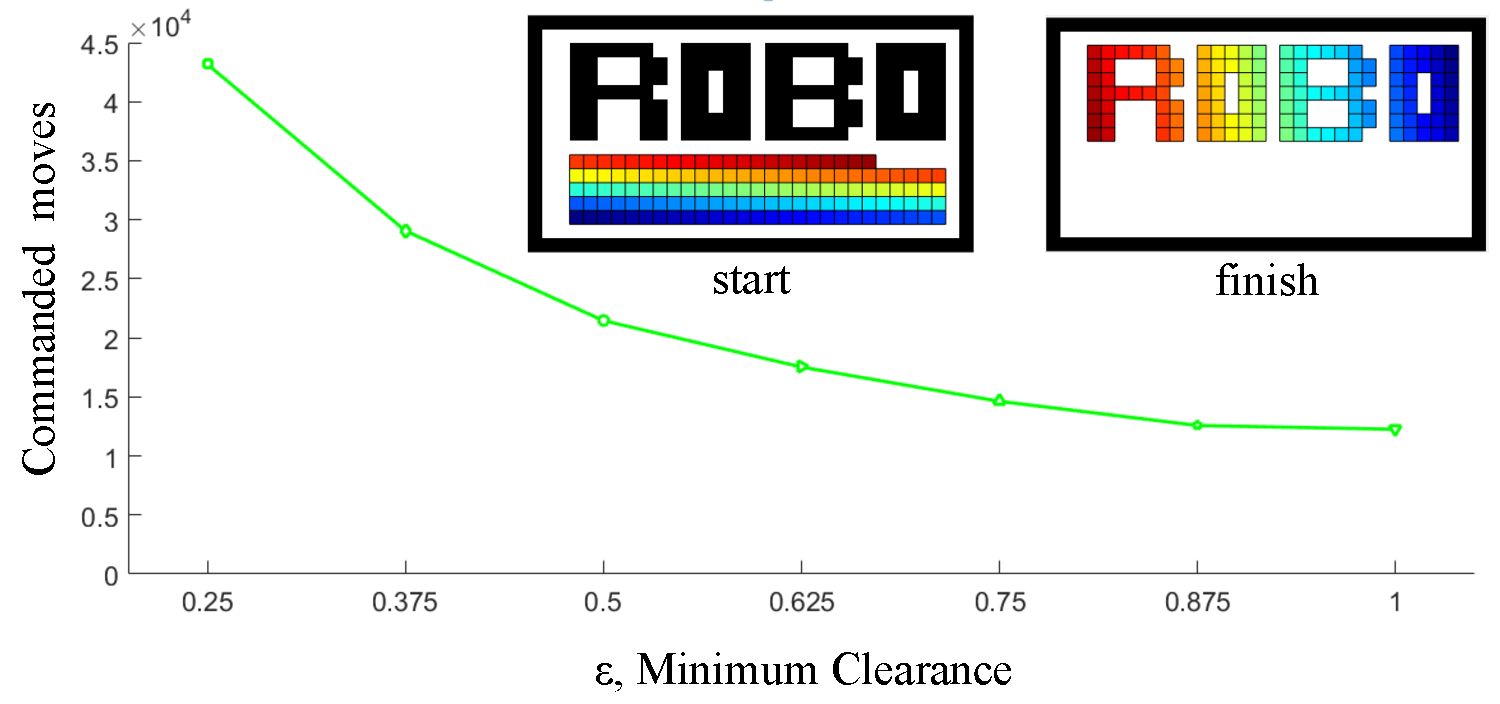
\includegraphics[width=\columnwidth]{graphrobo.pdf}
\end{center}
\caption{\label{fig:graphrobo.pdf}
Control performance is sensitive to the desired clearance $\epsilon$.  As $\epsilon$ increases, the total distance decreases asymptotically.
}
\end{figure}

\subsection{Efficient Control of Covariance}
A set of simulations were conducted to demonstrate the importance of boundary friction.  These simulations use  the 2D physics engine Box2D, by \citet{catto2010box2d}.
 144 disc-shaped robots were controlled by an open-loop control input.  All robots had  the same initial conditions, but in four tests the boundary friction was $F_f = \{0,1/3 F, 2/3F, F\}$.
 Without friction, covariance has minimal variation.  As friction increases, the covariance can be manipulated to greater degrees.


\begin{figure}
\begin{center}
	\includegraphics[width=\columnwidth]{SimCovarianceFuncFrictionOpenLoopV2.pdf}
\end{center}
\caption{\label{fig:SimCovarianceFuncFrictionOpenLoop}
Open-loop simulation with 144 disc robots and varying levels of boundary friction under the same initial conditions.  Without friction, covariance is unchangeable.  As friction increases, the covariance can be manipulated to greater degrees.
}
\end{figure}

 144 disc-shaped robots were also controlled by a closed-loop controller using  Alg.~\ref{alg:CovCont} with the same physics engine. Fig. \ref{fig:CovVarControlPlot} illustrates that covariance and variances in $x$ and $y$ axis were controlled.
\begin{figure}
\begin{center}
	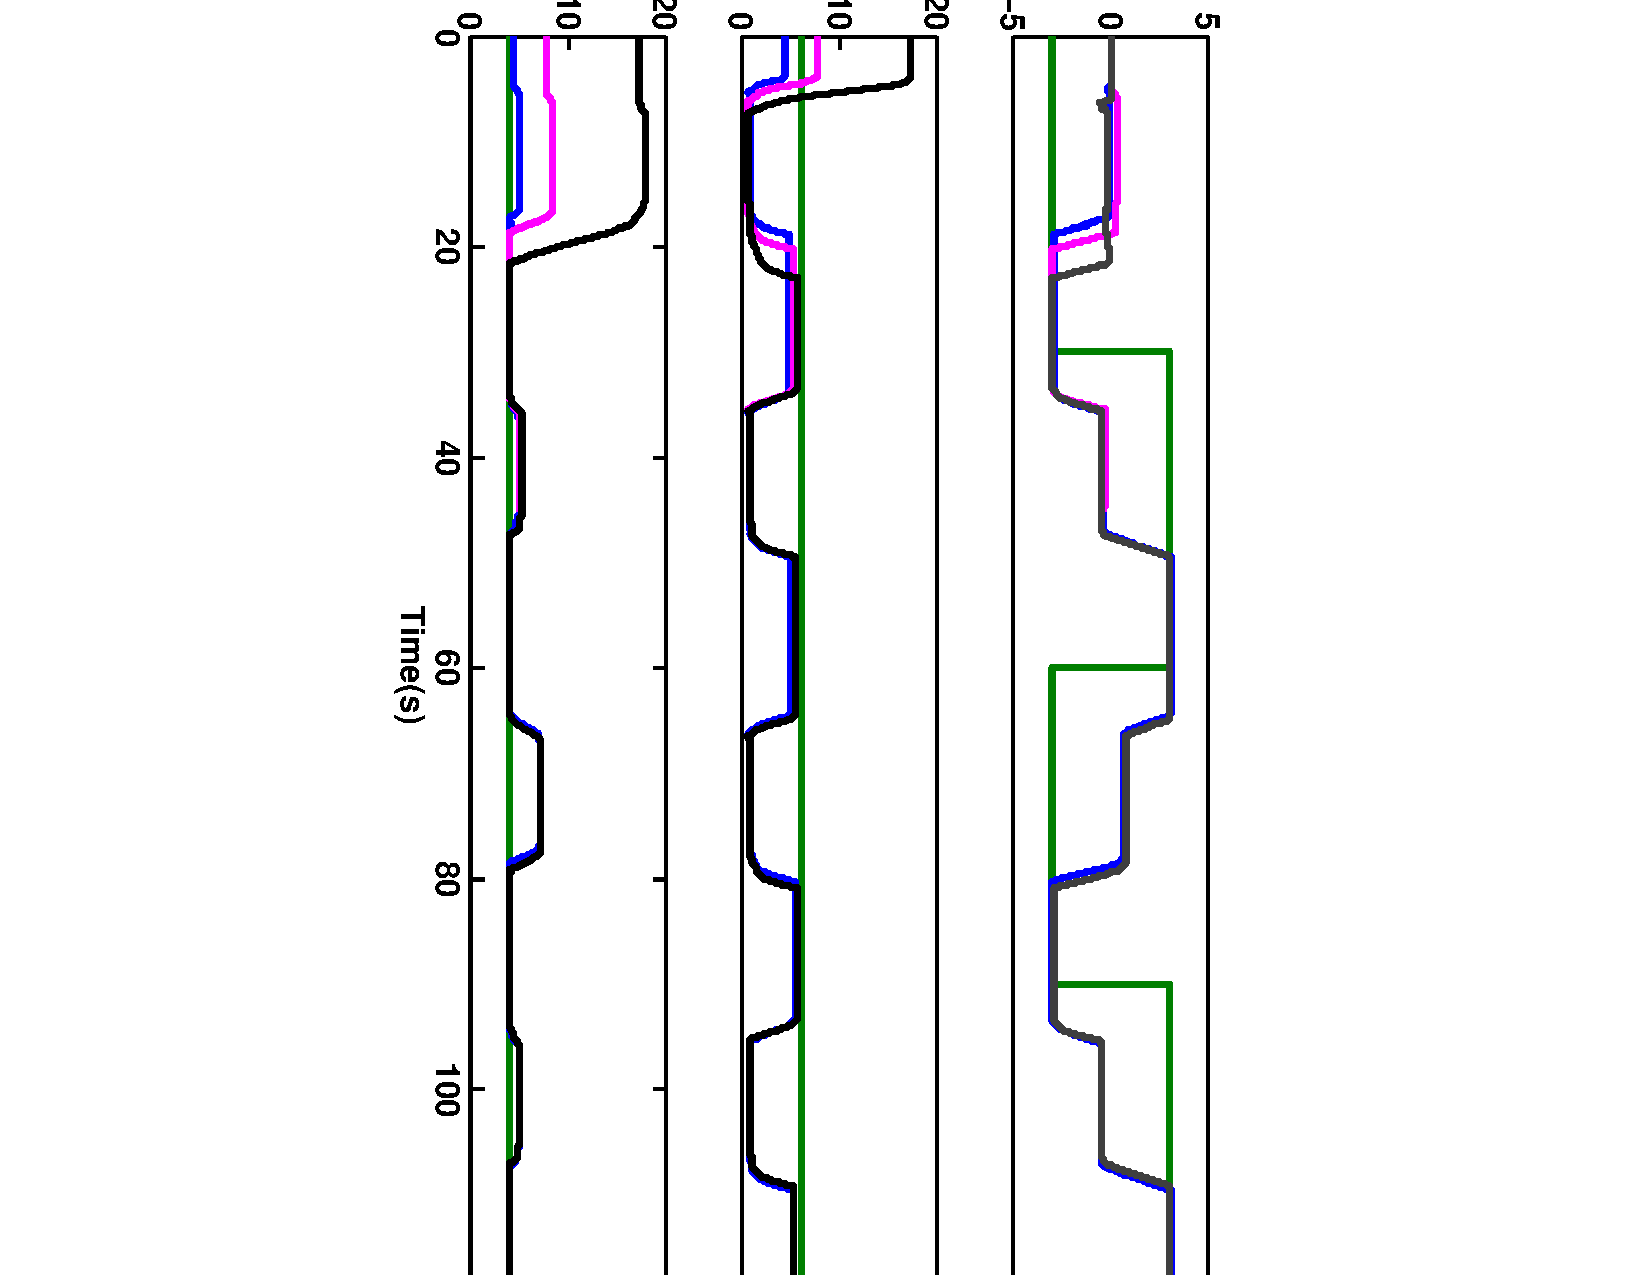
\includegraphics[width=\columnwidth]{CovVarControlPlot.pdf}
\end{center}
\caption{\label{fig:CovVarControlPlot}
Closed-loop simulation with 144 disc robots and three sets of initial conditions.  The algorithm tracks goal variance and covariance values (green).  The goal covariance switches sign every 30 s.}
\end{figure}


%%%%%%%%%%%%%%%
%%%%%%%%%%%%%%%
%
%%%%%%%%%%%%%%%%%%%%%%%%%%%%%%%%%%%%%%%%%%%%%%%%%%%%%%%%%%%
\section{Experiment}\label{sec:expResults}
%%%%%%%%%%%%%%%%%%%%%%%%%%%%%%%%%%%%%%%%%%%%%%%%%%%%%%%%%%%



\subsection{Hardware system}


Our experiments are on centimeter-scale hardware systems.  It allows us to emulate a variety of dynamics, while enabling a high degree of control over robot function, the environment, and data collection. The kilobot \cite{Rubenstein2012,rubenstein2014programmable} is a low-cost robot designed for testing collective algorithms with large numbers of robots. It is available commercially or as an open source platform~\cite{K-Team2015}.  Each robot is approximately 3 cm in diameter, 3 cm tall, and uses two vibration motors to move on a flat surface at speeds up to 1 cm/s.  Each robot has one ambient light sensor that is used to implement \emph{phototaxis},  moving towards a light source. 
In these experiments as shown in Fig.~\ref{fig:setup} , we used $n$=68 kilobots, a 1.5 m$\times$1.2 m whiteboard as the workspace, and four 30W LED floodlights arranged at the $\{N,E,S,W\}$ vertices of a 6 m square centered on the workspace. The lights were controlled by using an Arduino Uno board connected to an 8 relay shield board. Also at top of the table, an overhead machine vision system was added to track the position of the swarm.

\begin{figure}
\begin{center}
	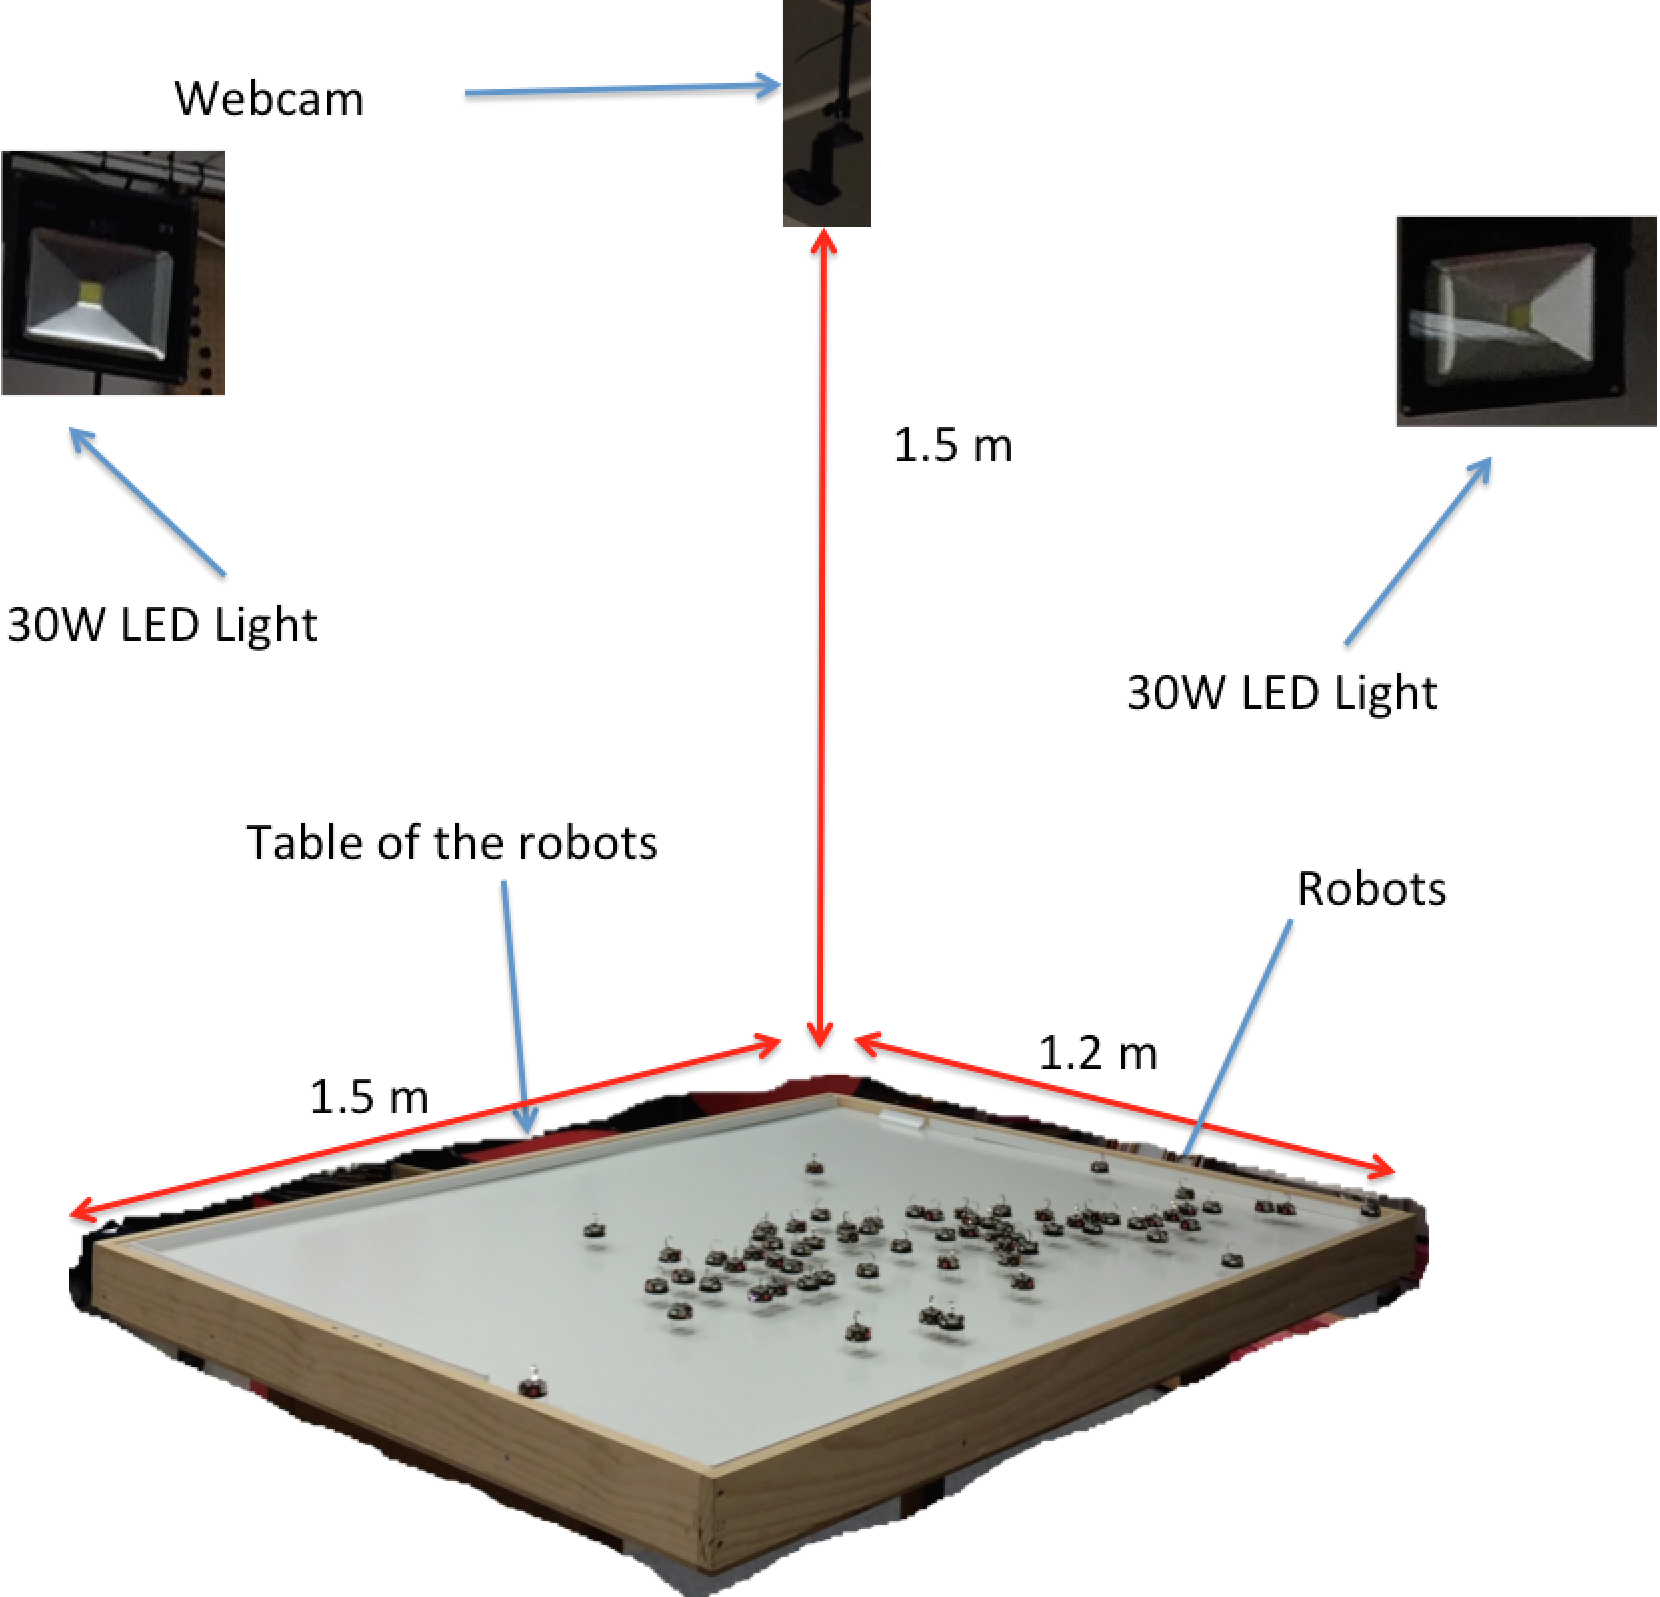
\includegraphics[width=\columnwidth*2/3]{SetUp.png}
\end{center}
\caption{\label{fig:setup}
Our workspace with a table of 1.5$\times$1.2 m and four 30W LED floodlights and an overhead machine vision system.
}
\end{figure}

The walls of the hardware platform have almost infinite friction, due mostly because the kilobots have three legs, so if the turn in one direction towards the wall, they will pin themselves to the wall until the light changes direction and they begin turning in the other direction.  This wall is sufficient to enable independent position control of two kilobots, as shown in Fig.~\ref{fig:storyReal}.



\begin{figure*}
\centering
\renewcommand{\figwid}{0.4\columnwidth}
{\begin{overpic}[width =\figwid]{twoR_1.png}\put(15,15){$t$  = 30 s}
\end{overpic}
\begin{overpic}[width =\figwid]{twoR_3.png}\put(15,15){$t$  = 60 s}
\end{overpic}
\begin{overpic}[width =\figwid]{twoR_2.png}\put(15,15){$t$  = 90 s}
\end{overpic}
\begin{overpic}[width =\figwid]{twoR_4.png}\put(15,15){$t$  = 120 s}
\end{overpic}
\begin{overpic}[width =\figwid]{twoR_5.png}\put(15,15){$t$  = 150 s}
\end{overpic}}
\vspace{-1em}
\caption{\label{fig:storyReal}{Two robot positioning using the hardware setup and two kilobot robots.  The walls have nearly infinite friction, as illustrated by the robot with the blue path that is stopped by the wall until the light changes orientation, while the orange robot in free-space is unhindered.}
%\vspace{-2em}
}
\end{figure*}


To demonstrate covariance control $n=68$ robots where placed on the workspace and manually steered with a single light source, using friction with the boundary walls to vary the covariance from  -5000 to 10,000.  The resulting covariance is plotted in Fig.~\ref{fig:covExperiment}, along with snapshots of the swarm.



\begin{figure}
\begin{center}
	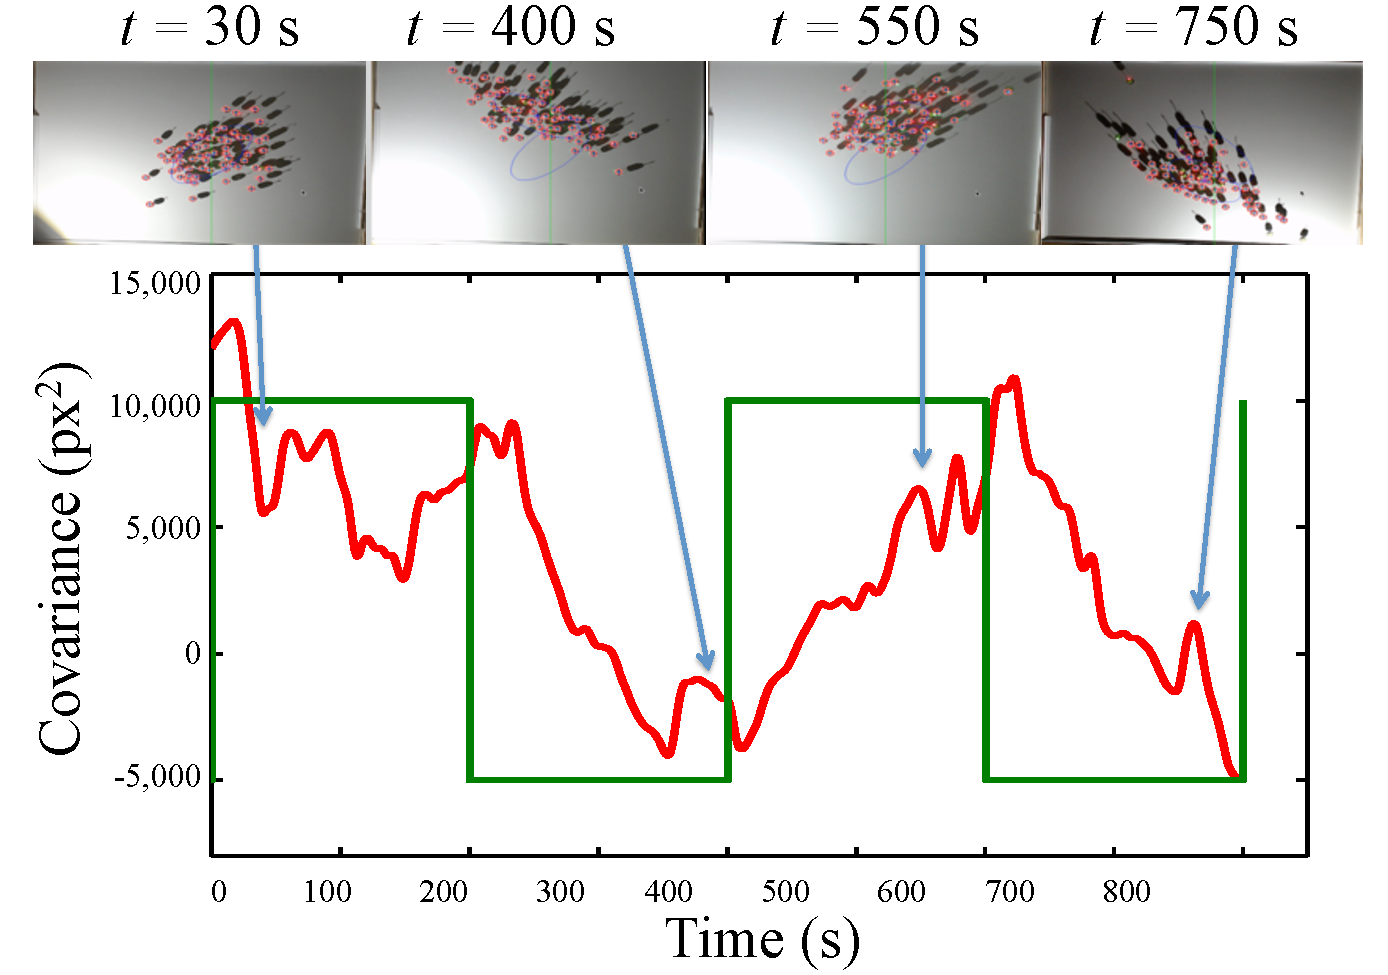
\includegraphics[width=\columnwidth]{experiment.pdf}
\end{center}
\caption{\label{fig:covExperiment}
Hardware demonstration steering 68 kilobot robots to desired covariance.  Frames above the plot show output from machine vision system and an overlaid covariance ellipse.
}
\end{figure}


%%%%%%%%%%%%%%%
%%%%%%%%%%%%%%%
%%%%%%%%%%%%%%%%%%%%%%%%%%%%%%%%%%%%%%%%%%%%%%%%%%%%%%%%%%%%
\section{Conclusion and Future Work}\label{sec:conclusion}
%%%%%%%%%%%%%%%%%%%%%%%%%%%%%%%%%%%%%%%%%%%%%%%%%%%%%%%%%%%


This paper presented techniques for controlling the orientation of an object by manipulating it using a swarm of simple robots with global inputs.
The paper provided algorithms for precise orientation control, as well as demonstrations of orientation control. 


Future efforts should be directed toward optimizing torque control, applying the techniques to hardware robots, pose control for multiple part assembly, and manipulation in a crowded workspace.
The control laws in this paper used only the mean and variance of the swarm.  The control techniques may be optimized using high-order moments, or by stochastic modeling of the collisions between swarm members and the object.

%TODO JOURNAL: design controllers that efficiently regulate $\sigma_{xy}$.
%TODO JOURNAL: We will design Lyapunov-inspired controllers for $\sigma_{xy}$ to prove controllability. 
%TODO JOURNAL:  and rank controllability as a function of friction.
% TODO: JOURNAL: and vary wall friction by laser-cutting boundary walls with a variety of profiles. 


%    Inspired by large-scale human experiments with swarms of robots under global control,  this paper investigated controllers that use only the mean and variance of a robot swarm. We proved that the mean position is controllable, and provided conditions under which variance is controllable.  We derived automatic controllers for each and a hysteresis-based switching control that controls the mean and variance of a robot swarm.  We employed these controllers as primitives for a block-pushing task. 
%    
%    Future work should implement these controllers on a robot swarm and decrease completion time by avoiding counter-productive contact with the block while the swarm is lowering its variance.  We have also assumed the swarm is unimodal and has a straight-line path to the moveable block. Relaxing these assumptions requires solving the \emph{gathering problem}.  The gathering problem for a swarm with uniform inputs is largely unexplored, and must be examined probabilistically for nontrivial environments.
%    
    % We should also control the covariance $\sigma_xy$ and higher moments of the distribution
    
    
    
%Sensing is expensive, especially on the nanoscale. To see nanocars~\cite{Chiang2011}, scientists fasten molecules that fluoresce light when activated by a strong light source. Unfortunately, multiple exposures can destroy these molecules, a process called \emph{photobleaching}. Photobleaching can be minimized by lowering the excitation light intensity, but this increases the probability of missed detections~\cite{Cazes2001}. A control methodology based on statistics of the robot swarm rather than the actual position of each robot, allows relaxing demands on imagine systems, controllers robust to tracking errors, and a simpler methodology.  In this work we...
%


% Additionally, as population characteristics, they are available even if only a percentage of the robots are detected each control cycle.
%Photobleaching: http://www.piercenet.com/browse.cfm?fldID=4DD9D52E-5056-8A76-4E6E-E217FAD0D86B
%
%Photobleaching is caused by the irreversible destruction of fluorophores due to either the prolonged exposure to the excitation source or exposure to high-intensity excitation light. Photobleaching can be minimized or avoided by exposing the fluor(s) to the lowest possible level of excitation light intensity for the shortest length of time that still yields the best signal detection; this requires optimization of the detection method using high sensitivity CCD cameras, high numerical aperture objective and/or the widest bandpass emission filter(s) available. Other approaches include using fluorophores that are more photostable than traditional fluorophores and/or using antifade reagents to protect the fluor(s) against photobleaching. Steps to avoid photobleaching are not feasible for all detection methods and should be optimized for each method used. For example, antifade reagents are toxic to live cells, and therefore they can only be used with fixed cells or tissue. Furthermore, some detection methods, such as flow cytometry, normally do not require steps to avoid photobleaching because of the extremely short exposure time of the fluorophore to the excitation source.
%%%%%%%%%%%%%%%


%\missingfigure[figwidth=6cm]{Intro: image of real vascular network}
%\missingfigure[figwidth=6cm]{Theory: Inkscape image showing how wall friction breaks symmetry caused by global inputs}
\missingfigure[figwidth=6cm]{Simulation: box2d example showing controlling the covariance of a swarm of 200 robots}
%\missingfigure[figwidth=6cm]{Simulation: mathematica demo showing control of the position of 2 robots}
\missingfigure[figwidth=6cm]{Experiment: image of testing environment: show table, 101 robots, camera, and 2 lights. }
\missingfigure[figwidth=6cm]{Time-lapse collage of robots changing covariance }
\missingfigure[figwidth=6cm]{Time-lapse collage of 2 robots changing their relative positions }

    
%\section{Acknowledgements}
%We acknowledge many \href{http://mrsl.rice.edu/}{mrsl.rice.edu} lab members who helped beta test \href{http://www.swarmcontrol.net}{SwarmControl.net}; helpful discussion with \href{http://www.jmtour.com/}{James Tour}, \href{http://slink.rice.edu/}{Stephan Link}, and Victor Garc\`ia L\`opez on fabrication and visualization challenges at the nanoscale with nanocars; and the \href{http://cttl.rice.edu/}{Rice Center for Technology in Teaching and Learning}.
%This work was partially supported by the National Science Foundation under 
%\href{http://www.nsf.gov/awardsearch/showAward?AWD_ID=1035716}{CPS-1035716}.  
   
\bibliographystyle{IEEEtran}
\bibliography{IEEEabrv,ShapingSwarmFrictionSharedInput}%,../../../ensemble/bib/aaronrefs}%,../aaronrefs}
\end{document}


%/Users/ab55/Desktop/svn/MRSL-Papers/Drafts-Current/2013-03-13-IROS-MassiveUniformManipulation/document
%/Users/ab55/Desktop/svn/ensemble/bib





